% Traceability: manual-local galactic field chapter.
\subsection{Galactic systems}

\subsubsection{Five-galaxy SPARC shell witness}
\label{man:five-galaxy-sparc-witness}
\colabbadge{manual/notebooks/04b_galactic_systems_sparc.ipynb}

\begin{table}[H]
\centering
\caption{Galactic retained-extraction declaration.}
\label{tab:galactic-retention}
\begin{threeparttable}
\begin{tabularx}{\linewidth}{@{}lX@{}}
\toprule
Item & Declaration \\
\midrule
Parent field & cited five-galaxy AO field family \\
Retained extraction & outer-orbital shell witness set \\
Omitted context & galaxy-internal contexts outside the reported shell record \\
First refinement & galaxy-specific full rotation row \\
Validity window & cited SPARC comparison window \\
Residual witness & pending until refinement rows are computed \\
\bottomrule
\end{tabularx}
\end{threeparttable}
\end{table}

The cited five-galaxy set is fixed first. The outer-orbital comparison is a source-normalized presentation of this witness layer. The public SPARC source is cited for the rotation-curve database and source quantities~\cite{sparc_paper,sparc_site}; a local snapshot used by \(\Phi_{\mathrm{SPARC}}\) must record its source units, version/access date, and normalization map before the calculated column is complete.

\begin{table}[H]
\centering
\caption{Five-galaxy SPARC cited row.}
\label{tab:five-galaxy-row}
\begin{threeparttable}
\small
\begin{tabularx}{\linewidth}{@{}lXcc@{}}
\toprule
Row & Structural class & $B^*$ & $\Lambda_b$ \\
\midrule
G1 & \texttt{tetron:*:[galaxy,star]:6} & 137 & 8 \\
\bottomrule
\end{tabularx}
\ManualTableNote{The shell-family and outer-orbital comparison are read on the same cited five-galaxy row.}
\end{threeparttable}
\end{table}

\begin{table}[H]
\centering
\caption{Five-galaxy outer-orbital comparison.}
\label{tab:five-galaxy-comparison}
\begin{threeparttable}
\small
\begin{tabularx}{\linewidth}{@{}lXcccc@{}}
\toprule
Map & Galaxy & Calculated [km/s] & Cited benchmark [km/s] & Abs. error [km/s] & Rel. error [\%] \\
\midrule
\(\Phi_{\mathrm{SPARC}}\) & NGC 2403 & pending & 134.4 & pending & pending \\
\(\Phi_{\mathrm{SPARC}}\) & NGC 3198 & pending & 149.2 & pending & pending \\
\(\Phi_{\mathrm{SPARC}}\) & NGC 6503 & pending & 115.6 & pending & pending \\
\(\Phi_{\mathrm{SPARC}}\) & NGC 2841 & pending & 288.2 & pending & pending \\
\(\Phi_{\mathrm{SPARC}}\) & DDO 154 & pending & 47.0 & pending & pending \\
\bottomrule
\end{tabularx}
\ManualTableNote{The SPARC source snapshot and \(\Phi_{\mathrm{SPARC}}\) normalization map must be explicit before the calculated column is complete.}
\end{threeparttable}
\end{table}

\begin{figure}[H]
\centering
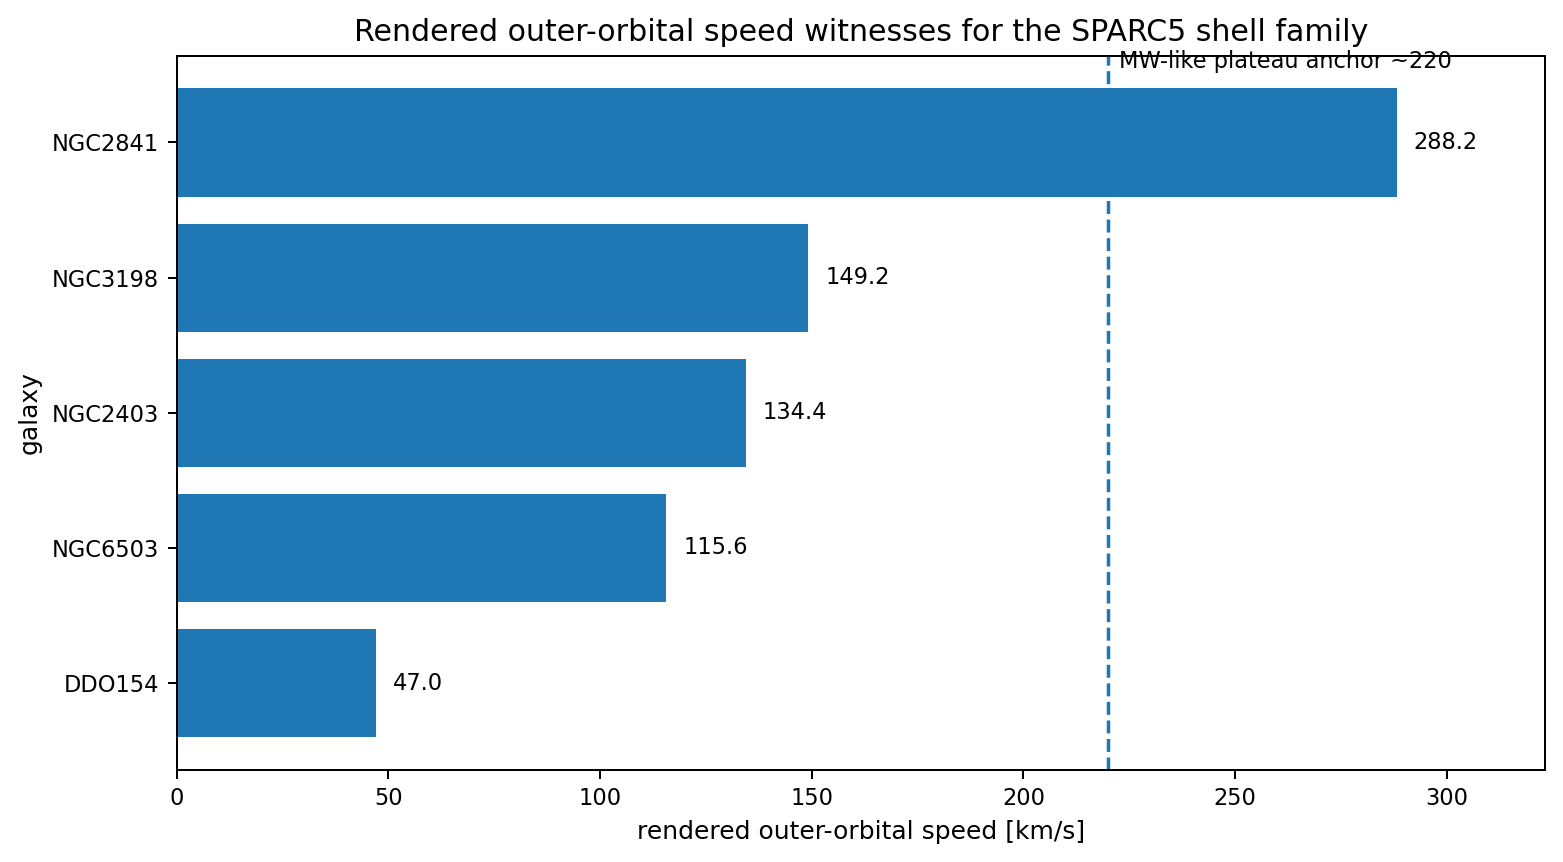
\includegraphics[width=0.88\linewidth]{figures/galactic/01_five_galaxy_comparison.png}
\caption{Five-galaxy outer-orbital comparison witness.}
\label{fig:five-galaxy-comparison}
\end{figure}

\begin{figure}[H]
\centering
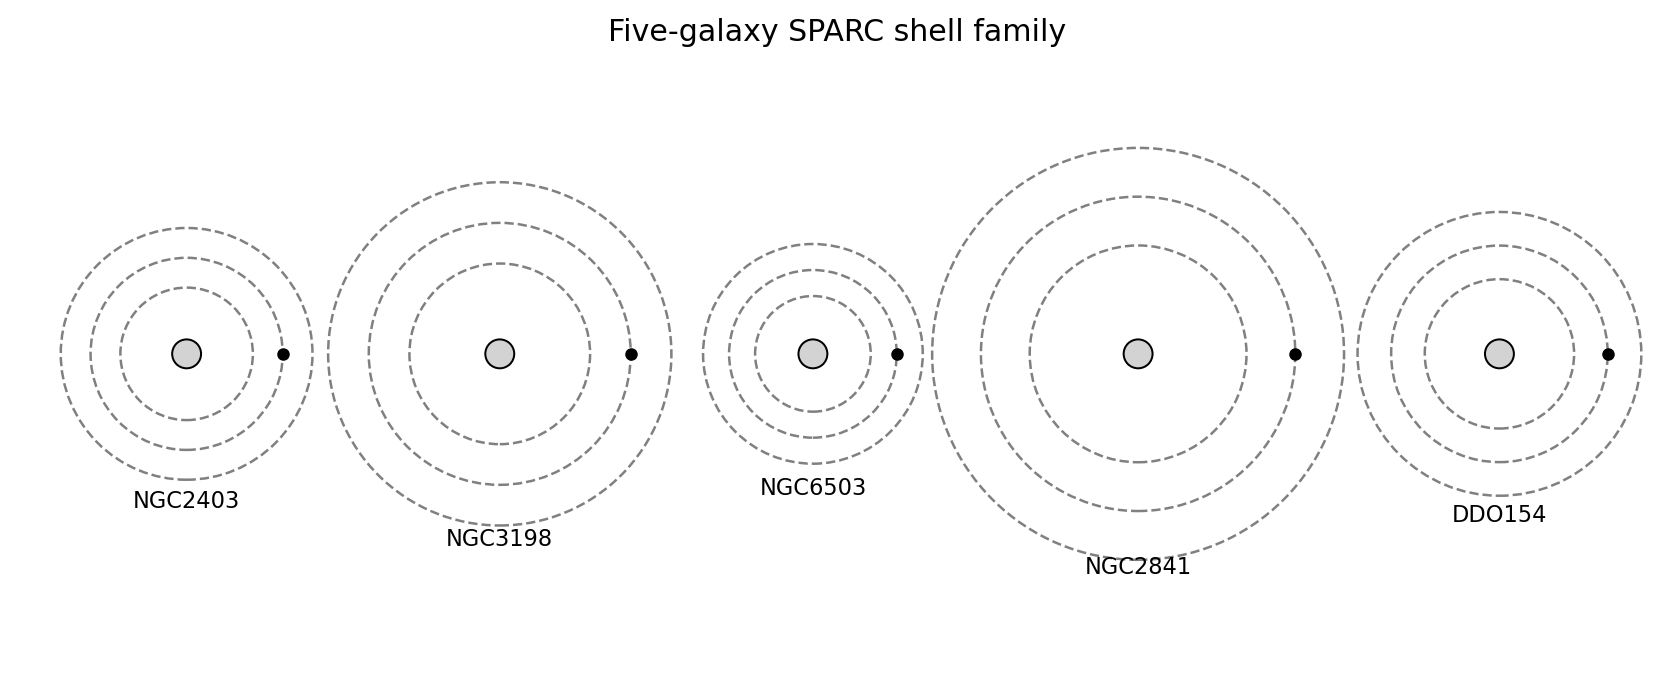
\includegraphics[width=0.88\linewidth]{figures/galactic/02_shell_family.png}
\caption{Five-galaxy shell-family schematic.}
\label{fig:five-galaxy-shell-family}
\end{figure}

The cited long-window record carries the shell-family witness together with the source-normalized five-galaxy comparison.
